\documentclass{scrartcl}
\usepackage[utf8]{inputenc}
\usepackage[a4paper, left=2cm, right=2cm, top=2cm, bottom=3cm]{geometry}
\usepackage{xcolor}
\usepackage{colortbl}
\usepackage{float}
\usepackage[export]{adjustbox} %bilder positionieren
% |-- mathematische Formeln
% |
\usepackage{amsmath, amsthm, amssymb, amsfonts}

%Mit Deckblattbild
\title{Ergonomic Posture Detection}
\author{Nourhan Omar, Vipin Singh, Polina Trump, Pavlo Kravets, Ari (Sara) Wahl }
\date{January 30th 2024
\begin{figure}[h]
    %\centering
    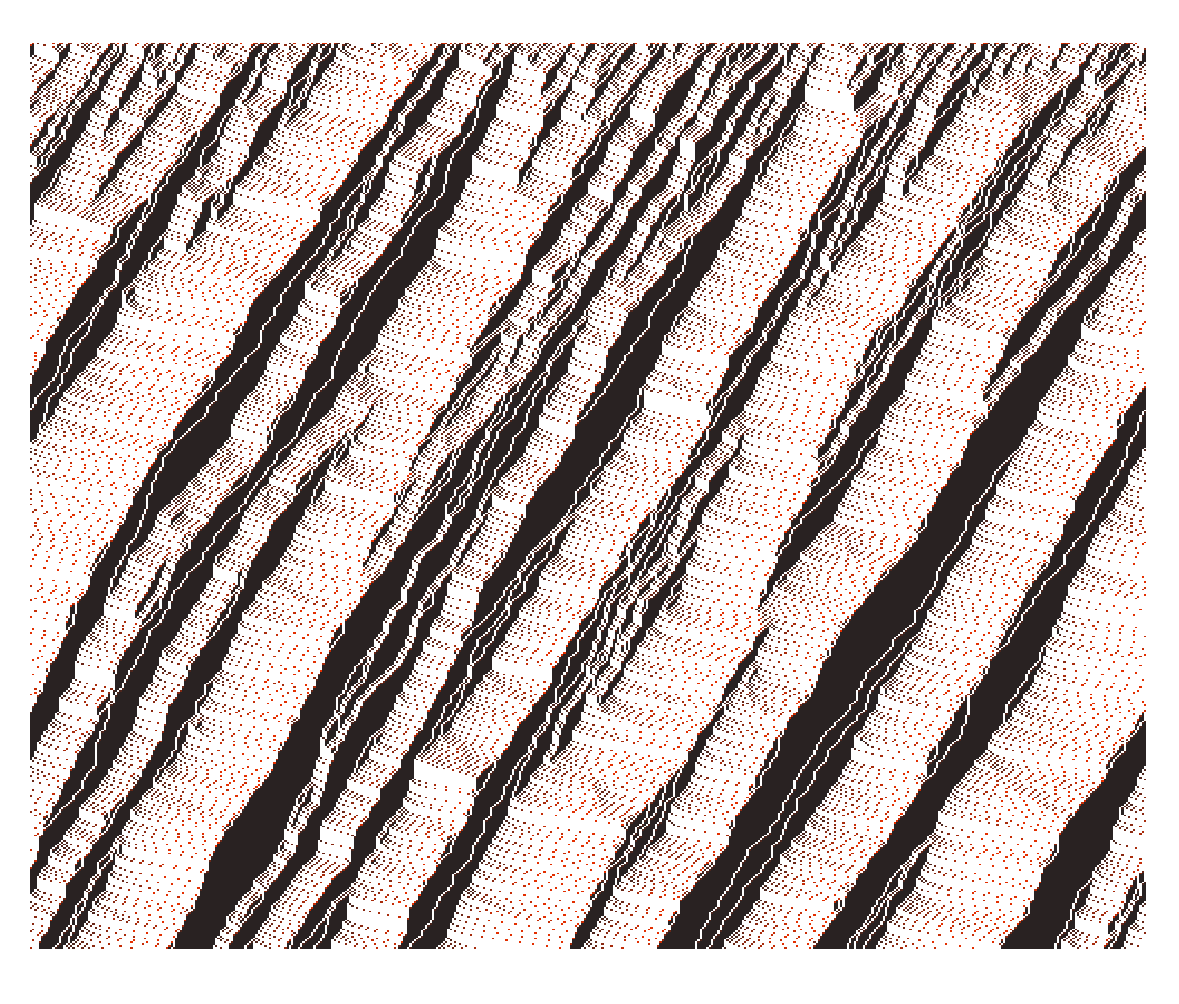
\includegraphics[width=17.5cm,height=17.5cm]{test.png}
\end{figure}
}

% |
% |-- Deutsche Buchstaben
% |
% +---- Kodierung
\usepackage[utf8]{inputenc}
\usepackage[T1]{fontenc}
\usepackage{lmodern}
% |
% +---- Sprache (neue deutsche Rechtschreibung)
% |
\usepackage[ngerman]{babel}

% |
% +---- Bilder in Grids

\usepackage{graphicx}
\usepackage{subcaption}
\graphicspath{{Images_LaTex_Report/}}

% +---- \usepackage{hyperref} -> be careful, usually, it has to be the last package to be imported, but there might be some exceptions to this rule
% |
\usepackage{hyperref}
\hypersetup{
    colorlinks=true,
    linkcolor=blue,
    filecolor=magenta,
    urlcolor=cyan,
}
\urlstyle{same}

\setlength\parindent{0pt} % Einrückung beim "paragraph" wegmachen am Anfang

%Source management with Biblatex

\usepackage[backend = biber, sorting=none]{biblatex}
\addbibresource{references.bib}
%\bibliographystyle{unsrt}  % Zitation in aufsteigender Reihenfolge 

\begin{document}
\maketitle

% +-----------------------------------------------------------------------------
% |
% |  Inhaltsverzeichnis
% |
% +-----------------------------------------------------------------------------
% |
\newpage
    \pagenumbering{roman}
    \begin{small}
    \tableofcontents
    \end{small}
\newpage
% |
% +-- reset the page numbering & change the style to arabic instead of roman
% |
\pagenumbering{arabic}

\section{Introduction}
\newpage
\section{Real Life Problem}
\newpage
\section{Technical Solution}
\newpage
\section{Business Model - how to capture value}
\newpage
\section{Technology - why is it unique}
\newpage
\section{Marketing}
\newpage
\section{Competition}
\newpage
\input{Status or timeline: where are you now, what next}
\newpage
\section{Team}
\newpage
\section{Business Model Canvas}
\newpage
\section{Planned Figures}
\newpage
\section{Executive Summary}
\newpage
\addcontentsline{toc}{section}{Literatur}
\printbibliography

\end{document}